\documentclass{./../div_teaching_slides}

\begin{document}
\title{ECON 340 \\ Economic Research Methods}
\author{Div Bhagia}
\date{Lecture 13: Confidence Intervals}

%%%%%%%%%%%% 
\begin{frame}[noframenumbering, plain]
\maketitle
\end{frame}


%%%%%%%%%%%%
\begin{frame}{Expectation and Variance of $\bar{X}$}
Let $X_1,X_2,...,X_n$ denote independent random draws (random sample) from a population with mean $\mu$ and variance $\sigma^2$. 
$$ \bar{X} = \frac{1}{n} \sum_{i=1}^n X_i $$
Then $\bar{X}$ is also a random variable with:
$$E(\bar{X}) = \mu \quad \quad \quad  \sigma^2_{\bar{X}}= \frac{\sigma^2}{n} $$ 

So $\bar{X}$ is an unbiased and consistent estimator for $\mu$.
\end{frame}

%%%%%%%%%%%%
\begin{frame}{Sample Mean Distribution}
The distribution of the sample mean is \underline{normal} if \textit{either} of the following is true: \\~\\
\begin{witemize}
  \item The underlying population is normal
  \item The sample size is large, say $n\geq 100$ \\~\\
\end{witemize}
The first one follows from the sample mean being a linear combination of normally distributed variables. \\~\\

The latter is implied by the \textit{Central Limit Theorem}. 
\end{frame}

%%%%%%%%%%%%
\begin{frame}{Central Limit Theorem}
\vspace{2em}
If $X_1, X_2,..,X_n$ are drawn randomly from a population with mean $\mu$ and variance $\sigma^2$, sample mean $\bar{X}$ is normally distributed with mean $\mu$ and variance $\sigma^2/n$ as long as $n$ is large.
$$\bar{X} \sim N\left(\mu, \dfrac{\sigma^2}{n}\right)$$ \\~\\
\href{https://dbhagia.shinyapps.io/CLT-Demo/}{\blue{Simulation}}
\end{frame}

%%%%%%%%%%%%
\begin{frame}{Normal Distribution}
\vspace{-0.35em} 
95\% of the area under the curve lies within 1.96 standard deviations of the true mean. 
\vspace{1.7em} 

\centering
\begin{tikzpicture}
\begin{axis}[
  no markers, domain=-3:3, samples=100,
  axis lines*=left, xlabel=$\bar{X}$, ylabel=$f(\bar{X})$,
  %every axis y label/.style={at=(current axis.above origin),anchor=south},
  height=6cm, width=12cm,
  xtick={-1.96, 0, 1.96}, xticklabels={$\mu-1.96 \sigma_{\bar{X}}$, $\mu$, $\mu+1.96 \sigma_{\bar{X}}$}, %ytick=\empty,
  enlargelimits=false, clip=false, axis on top,
  ]
  \addplot [very thick,black] {gauss(0, 1)}; 
  \addplot [fill=purple!20, draw=none, domain=-1.96:1.96] {gauss(0, 1)} \closedcycle;
%\draw[->, line width=1pt](axis cs: 185, 0.0125)--(axis cs: 205, 0.0125);
\node at (axis cs: 0, 0.2) { 95\%};
\end{axis}
\end{tikzpicture} \\
\end{frame}

%%%%%%%%%%%%
\begin{frame}{Aside}
\vspace{-1em}
\centering
Standard Normal $\rightarrow$ Normal Distribution \\ \vspace{0.5em}

% Row 1
\begin{columns}[T]
\begin{column}{0.35\textwidth}
\begin{tikzpicture}[scale=0.5]
\begin{axis}[
  no markers, domain=-3:3, samples=100,
  axis lines*=left, xlabel=Z, ylabel=$f(Z)$,
  %every axis y label/.style={at=(current axis.above origin),anchor=south},
  height=6.5cm, width=12cm,
  xtick={-1.64, 0, 1.64}, %ytick=\empty,
  enlargelimits=false, clip=false, axis on top,
  ]
  \addplot [very thick,black] {gauss(0, 1)}; 
  \addplot [fill=purple!20, draw=none, domain=-1.64:1.64] {gauss(0, 1)} \closedcycle;
%\draw[->, line width=1pt](axis cs: 185, 0.0125)--(axis cs: 205, 0.0125);
\node at (axis cs: 0, 0.2) {90\%};
\end{axis}
\end{tikzpicture} 
\end{column}	
\begin{column}{0.1\textwidth}
\[
\xrightarrow{\hspace{1cm}}
\]
\end{column}
\begin{column}{0.45\textwidth}
\begin{tikzpicture}[scale=0.5]
\begin{axis}[
  no markers, domain=-3:3, samples=100,
  axis lines*=left, xlabel=X, ylabel=$f(X)$,
  %every axis y label/.style={at=(current axis.above origin),anchor=south},
  height=6cm, width=12cm,
  xtick={-1.64, 0, 1.64}, xticklabels={$\mu-1.64 \sigma_X$, $\mu$, $\mu+1.64 \sigma_X$}, %ytick=\empty,
  enlargelimits=false, clip=false, axis on top,
  ]
  \addplot [very thick,black] {gauss(0, 1)}; 
  \addplot [fill=purple!20, draw=none, domain=-1.64:1.64] {gauss(0, 1)} \closedcycle;
%\draw[->, line width=1pt](axis cs: 185, 0.0125)--(axis cs: 205, 0.0125);
\node at (axis cs: 0, 0.2) { 90\%};
\end{axis}
\end{tikzpicture}
\end{column}	
\end{columns} 
\vspace{1.5em}

% Row 2
\begin{columns}[T]
\begin{column}{0.35\textwidth}
\begin{tikzpicture}[scale=0.5]
\begin{axis}[
  no markers, domain=-3:3, samples=100,
  axis lines*=left, xlabel=Z, ylabel=$f(Z)$,
  %every axis y label/.style={at=(current axis.above origin),anchor=south},
  height=6.5cm, width=12cm,
  xtick={-1.96, 0, 1.96}, %ytick=\empty,
  enlargelimits=false, clip=false, axis on top,
  ]
  \addplot [very thick,black] {gauss(0, 1)}; 
  \addplot [fill=purple!20, draw=none, domain=-1.96:1.96] {gauss(0, 1)} \closedcycle;
%\draw[->, line width=1pt](axis cs: 185, 0.0125)--(axis cs: 205, 0.0125);
\node at (axis cs: 0, 0.2) {95\%};
\end{axis}
\end{tikzpicture} 
\end{column}	
\begin{column}{0.1\textwidth}
\[
\xrightarrow{\hspace{1cm}}
\]
\end{column}
\begin{column}{0.45\textwidth}
\begin{tikzpicture}[scale=0.5]
\begin{axis}[
  no markers, domain=-3:3, samples=100,
  axis lines*=left, xlabel=X, ylabel=$f(X)$,
  %every axis y label/.style={at=(current axis.above origin),anchor=south},
  height=6cm, width=12cm,
  xtick={-1.96, 0, 1.96}, xticklabels={$\mu-1.96 \sigma_X$, $\mu$, $\mu+1.96 \sigma_X$}, %ytick=\empty,
  enlargelimits=false, clip=false, axis on top,
  ]
  \addplot [very thick,black] {gauss(0, 1)}; 
  \addplot [fill=purple!20, draw=none, domain=-1.96:1.96] {gauss(0, 1)} \closedcycle;
%\draw[->, line width=1pt](axis cs: 185, 0.0125)--(axis cs: 205, 0.0125);
\node at (axis cs: 0, 0.2) { 95\%};
\end{axis}
\end{tikzpicture}
\end{column}	
\end{columns}
\end{frame}

%%%%%%%%%%%%
\begin{frame}{Normal Distribution}
\vspace{-0.35em} 
95\% of the time that we take a sample and calculate the sample mean, it will be within 1.96 standard deviations of $\mu$.
\vspace{1.7em} 

\centering
\begin{tikzpicture}
\begin{axis}[
  no markers, domain=-3:3, samples=100,
  axis lines*=left, xlabel=$\bar{X}$, ylabel=$f(\bar{X})$,
  %every axis y label/.style={at=(current axis.above origin),anchor=south},
  height=6cm, width=12cm,
  xtick={-1.96, 0, 1.96}, xticklabels={$\mu-1.96 \sigma_{\bar{X}}$, $\mu$, $\mu+1.96 \sigma_{\bar{X}}$}, %ytick=\empty,
  enlargelimits=false, clip=false, axis on top,
  ]
  \addplot [very thick,black] {gauss(0, 1)}; 
  \addplot [fill=purple!20, draw=none, domain=-1.96:1.96] {gauss(0, 1)} \closedcycle;
%\draw[->, line width=1pt](axis cs: 185, 0.0125)--(axis cs: 205, 0.0125);
\node at (axis cs: 0, 0.2) { 95\%};
\end{axis}
\end{tikzpicture} \\
\end{frame}

%%%%%%%%%%%%
\begin{frame}{Confidence Intervals}
\begin{witemize}
  \item If 95\% of the time, the sample mean $\bar{X}$ will be within 1.96 standard deviations of the true mean $\mu$.
  \item Then 95\% of the time, the true mean $\mu$ will be within 1.96 standard deviations of the sample mean $\bar{X}$.
  \item Use this logic to create a 95\% confidence interval for the true population mean $\mu$. 
  \item Say in your sample you found sample mean $\bar{x}$, then 95\% confidence interval for $\mu$:
  $$ \bar{x} \pm 1.96 \sigma_{\bar{X}} $$
\end{witemize}
\end{frame}

%%%%%%%%%%%%
\begin{frame}{Confidence Intervals: Interpretation}
\vfill
There is a 95\% chance that the true population average lies in the interval $ \bar{x} \pm 1.96 \sigma_{\bar{X}} $. \\~\\

What this really means is that if we took 100 random samples from the population and calculated 95\% confidence intervals for each sample, we would expect 95 out of 100 intervals to contain the true population mean.
\vfill
\end{frame}

%%%%%%%%%%%%
\begin{frame}{Confidence Intervals: Interpretation}
\centering
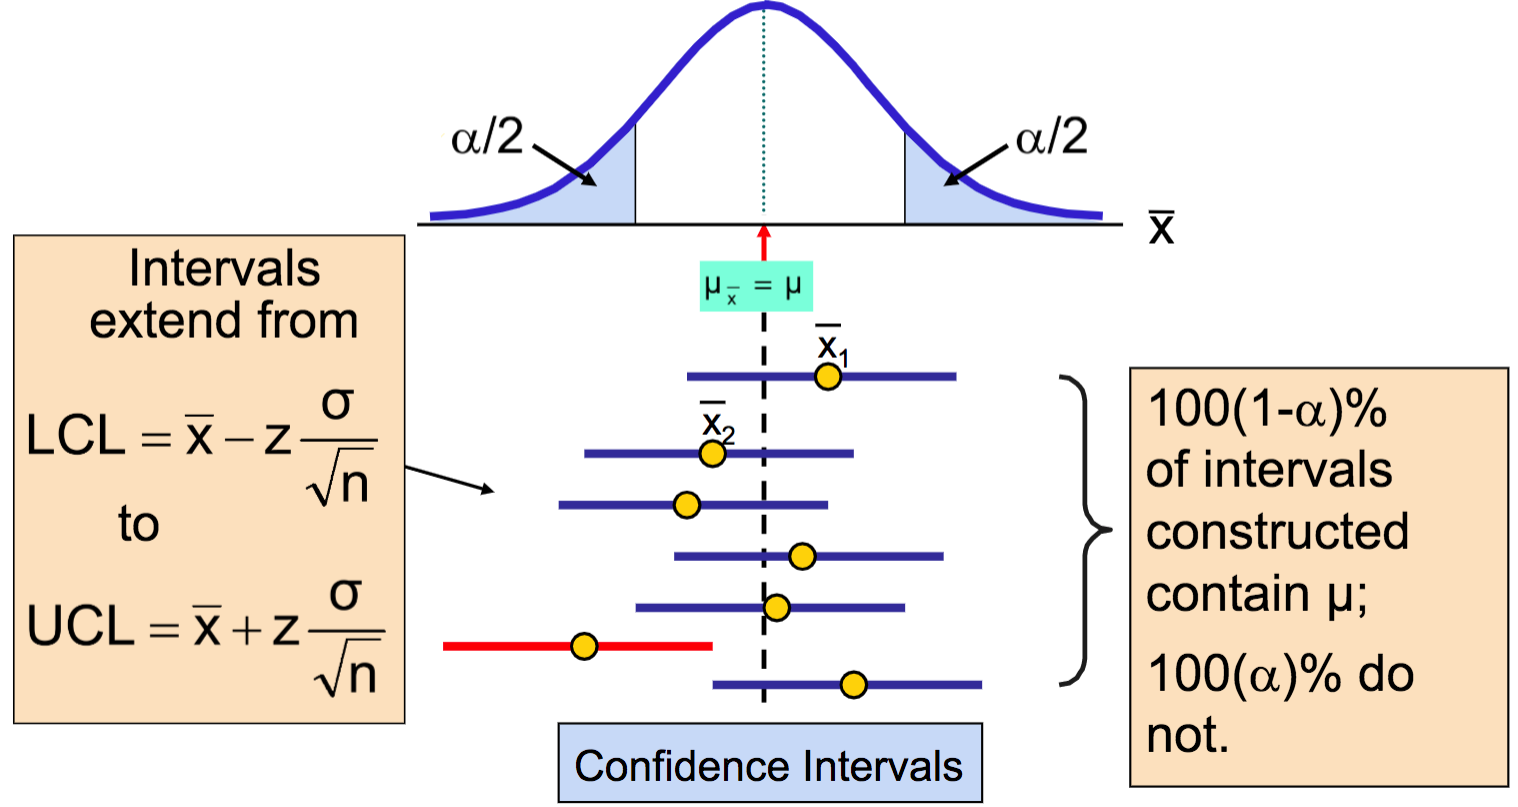
\includegraphics[scale=0.5]{ci_int.png}	
\end{frame}


%%%%%%%%%%%%
\begin{frame}{Recipe: Confidence Intervals}
Let $z_{\alpha/2}$ be the $z$-value that leaves area $\alpha/2$ in the upper tail of the normal distribution. \\~\\
Then $1-\alpha$ confidence interval is given by 
$$ \bar{x} \pm  \underbrace{z_{\alpha/2}  \frac{\sigma}{\sqrt{n}}}_{\text{Margin of Error}} $$
\end{frame}

%%%%%%%%%%%%
\begin{frame}{Margin of Error}
The margin of error will be reduced if \\~\\
\begin{itemize}
\item Population standard deviation is reduced $(\downarrow \sigma)$ \\~\\
\item The sample size is increased $(\uparrow n)$  \\~\\
\item The confidence level is decreased $(\downarrow (1-\alpha))$  \\~\\
\end{itemize}
\end{frame}

%%%%%%%%%%%%
\begin{frame}{Population variance is not known!}
\begin{witemize}
  \item So far, we have assumed that we know the true population variance $\sigma^2$
  \item This is obviously not realistic!
  \item Most times we have to use the sample variance $S^2$ instead of $\sigma^2$. 
  \item How do we create a confidence interval in this case?
\end{witemize}
\end{frame}

%%%%%%%%%%%%
\begin{frame}{Population variance is not known}
Instead of the $Z$ statistic, we can use the $T$ statistic
$$ T = \frac{\bar{X}-\mu}{S/\sqrt{n}} \sim t_{n-1} $$ 
It can be shown that this statistic follows a $t$ distribution with $n-1$ degrees of freedom. \\~\\
The t-distribution is similar to the normal distribution but has thicker tails to account for the greater uncertainty in smaller samples. However, in large samples $t$-distribution can be approximated by the standard-normal.
\end{frame}

%%%%%%%%%%%%
\begin{frame}{Student's T Distribution}
\centering
	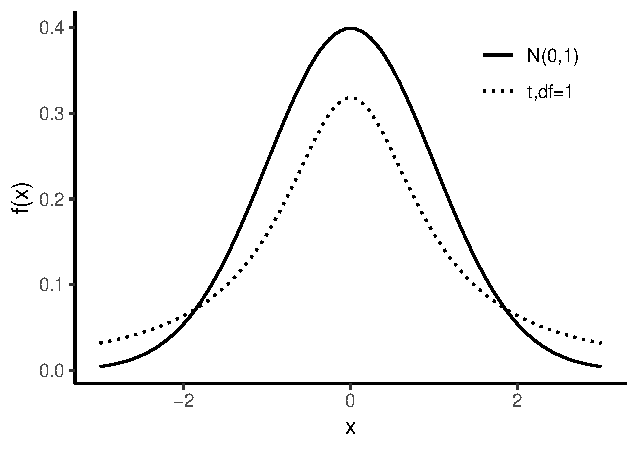
\includegraphics{./../../Output/tdist1.pdf} 
\end{frame}

%%%%%%%%%%%%
\begin{frame}{Student's T Distribution}
\centering
	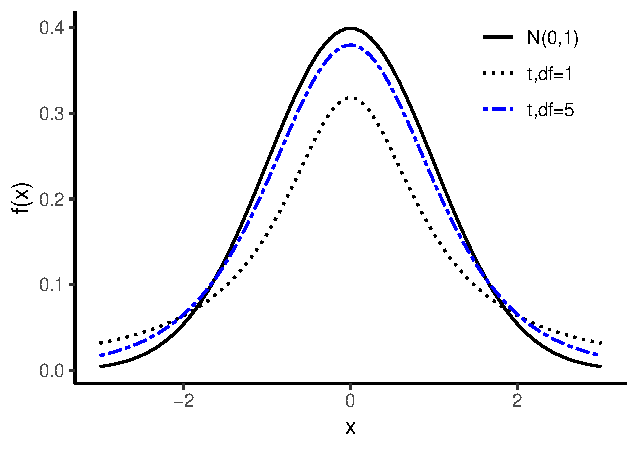
\includegraphics{./../../Output/tdist2.pdf} 
\end{frame}

%%%%%%%%%%%%
\begin{frame}{Student's T Distribution}
\centering
	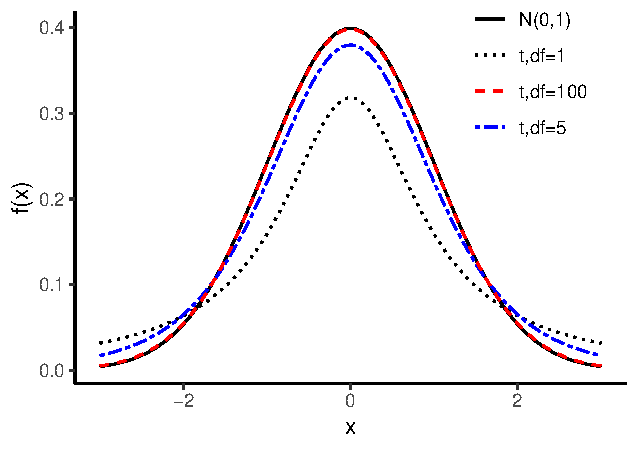
\includegraphics{./../../Output/tdist.pdf} 
\end{frame}

%%%%%%%%%%%%
\begin{frame}{Confidence Intervals: Unknown Variance}
\begin{witemize}
  \item Construct the confidence interval as before but now use $T$ statistic instead of $Z$
  \item So need to use critical value for $t$
  $$ \bar{x} \pm  t_{\alpha/2,n-1}  \frac{S}{\sqrt{n}}$$
 \item But since we said that in large samples, $t$ is approximated by $z$, we can continue using the standard normal table for the critical values if $n \geq 100$. 
\end{witemize}
\end{frame}


%%%%%%%%%%%%
\begin{frame}{Next up}
\vspace{-0.5em}
\begin{witemize}
  \item Problem Set 3 is due by the end of the day today 
  \item Next class: Hypothesis testing and p-values
  \item Next week: \\
  \begin{witemize}
  \normalsize
  \item Review class on Tuesday 
  \item Midterm exam on Thursday 
\end{witemize}
\end{witemize}
\end{frame}




\end{document}